%Master File:lectures.tex

\lesson{Vector Spaces}
\vspace{-2cm}
\begin{center}
  \setlength{\unitlength}{1bp}
  \begin{picture}(500,200)
    \put(0,40){\textcolor{red}{\begin{rotate}{15}$\displaystyle
          \begin{pmatrix}
            1 & 1 & 1 & 1 & 1 \\
            1 & 2 & 4 & 8 & 16 \\
            1 & 3 & 9 & 27 & 81 \\
            1 & 4 & 16 & 64 & 256 \\
            1 & 5 & 25 & 125 & 625
          \end{pmatrix}
          \begin{pmatrix}
            a_0 \\ a_1 \\ a_2 \\ a_3 \\ a_4
          \end{pmatrix}
          =
          \begin{pmatrix}
            1 \\ 1 \\ 2 \\ -3 \\ 1
          \end{pmatrix}$\end{rotate}}}
    \put(180,30){\textcolor{green}{\begin{rotate}{-15}$\displaystyle
          \bm{\nabla}_{\mat{X}} \mathrm{Tr} (\mat{X}^{-1} \mat{A})
          = -\mat{X}^{-1} \mat{A}\mat{X}^{-1}$\end{rotate}}}
    \put(50,-100){\includegraphics[width=18cm]{linalg.eps}}
  \end{picture}
\end{center}
\keywords{Vectors, vector spaces, operators}

%%%%%%%%%%%%%%%%%%%%%%% Next Slide %%%%%%%%%%%%%%%%%%%%%%%
\renewcommand{\Outline}{%
\begin{slide}
\section[1]{Outline}

\begin{minipage}{12cm}
  \begin{enumerate}\squeeze
    \outlineitem{Vector Spaces}{vectorspaces}
    \outlineitem{Operators}{operators}
  \end{enumerate}
\end{minipage}\hfill
\begin{minipage}{10cm}
  \includegraphics[height=10cm]{linalg}
\end{minipage}
\end{slide}
\addtocounter{outlineitem}{1}
}

\setcounter{outlineitem}{1}

%%%%%%%%%%%%%%%%%%%%%%% Next Slide %%%%%%%%%%%%%%%%%%%%%%%
\Outline % Vector Spaces
\toptarget{firstoutline}
%%%%%%%%%%%%%%%%%%%%%%% Next Slide %%%%%%%%%%%%%%%%%%%%%%%

\begin{slide}
\section[-1]{Matrices, Vectors and All That}

\begin{PauseHighLight}
  \begin{itemize}
  \item The language of machine learning is mathematics\pause
  \item Sometimes we draw pretty pictures to explain the mathematics\pause
  \item Much of the mathematics we will use involves vectors, matrices
    and functions\pause
  \item You need to master the language of mathematics, otherwise you
    won't understand the algorithms\pause
  \item I'm going to spend this lecture and the next revising the
    mathematics you need to know\pause{} (but I'm going use a slightly posher
    language than you are probably used to)\pauseb
  \end{itemize}
\end{PauseHighLight}

\end{slide}

%%%%%%%%%%%%%%%%%%%%%%% Next Slide %%%%%%%%%%%%%%%%%%%%%%%

\begin{slide}
\section[-2]{Vectors}

\begin{PauseHighLight}
  \begin{itemize}
  \item We often work with objects with many components (features)\pause
  \item To help handle this we will use vector notation\pause
  \end{itemize}
  \begin{minipage}{0.29\linewidth}
    \begin{align*}
      \bm{x} =
      \begin{pmatrix}
        x_1 \\ x_2 \\ \vdots \\ x_n
      \end{pmatrix}\pause
    \end{align*}
  \end{minipage}
  \begin{minipage}{0.69\linewidth}
    \begin{itemize}
    \item We represent vectors by bold symbols\pause
    \item All our vectors are column vectors by default\pause
    \item We treat them as $n\times 1$ matrix\pause
    \end{itemize}
  \end{minipage}
  \begin{itemize}
  \item We write row vectors as transposes of column vectors
    \begin{align*}
      \bm{y}^\tr = (y_1, y_2, \ldots, y_n)\pause
    \end{align*}
  \end{itemize}
\end{PauseHighLight}
\end{slide}


%%%%%%%%%%%%%%%%%%%%%%% Next Slide %%%%%%%%%%%%%%%%%%%%%%%

\begin{slide}
\section[-2]{Basic Vector Operations}

\pb
\begin{itemize}
\item The basic vector operations are adding\pauseh\pauselevel{=1}
  \begin{center}
    \multipdf[width=0.4\linewidth]{addingVectors}\pause
  \end{center}
\item multiplying by a scalar (a number)\pauseh\pauselevel{=5}
  \begin{center}
    \multipdf[width=0.5\linewidth]{multiplyVector}\pause
  \end{center}
\end{itemize}

\end{slide}

%%%%%%%%%%%%%%%%%%%%%%% Next Slide %%%%%%%%%%%%%%%%%%%%%%%

\begin{slide}
\section[-1]{Vector Space}

\begin{PauseHighLight}
  \begin{itemize}
  \item A vector space, $\mathcal{V}$, is a set of vectors which satisfies
    \begin{enumerate}\squeeze
    \item if $\bm{v}, \bm{w}\in\mathcal{V}$ then
      $a\,\bm{v}\in\mathcal{V}$ and $\bm{v}+\bm{w}\in\mathcal{V}$\hfill
      (closure)\pause 
    \item $\bm{v} + \bm{w} = \bm{w} + \bm{v}$\hfill (commutativity of
      addition)\pause 
    \item $(\bm{u}+\bm{v}) + \bm{w} = \bm{u} + (\bm{v} + \bm{w})$\hfill
      (associativity of addition)\pause
    \item $\bm{v} + \bm{0} = \bm{v}$ \hfill(existence of additive identity
      $\bm{0}$)\pause 
    \item $1 \, \bm{v} = \bm{v}$\hfill (existence of multiplicative identity
      $1$)\pause
    \item $a\,(b\,\bm{v}) = (a\,b)\,\bm{v}$\hfill (distributive properties)
    \item $a\,(\bm{v} + \bm{w}) = a\,\bm{v} + a\,\bm{w}$
    \item $(a+b)\,\bm{v} = a\,\bm{v} + b\,\bm{v}$\pause
    \end{enumerate}
    (You don't need to remember these)\pause
  \item Just from these properties we can deduce other properties\pause
  \end{itemize}
\end{PauseHighLight}


\end{slide}

%%%%%%%%%%%%%%%%%%%%%%% Next Slide %%%%%%%%%%%%%%%%%%%%%%%

\begin{slide}
\section[-1]{$\mathbb{R}^n$}

\begin{PauseHighLight}
  \begin{minipage}{0.8\linewidth}
    \begin{itemize}
    \item When we first learn about vectors we think of them arrows in 3-D
      space\pause
    \item If we centre them all at the origin then there is a one-to-one
      correspondence between vectors and points in space\pause
    \item We call this vector space $\mathbb{R}^3$\pause
    \item Any set of quantities $\bm{x} = (x_1, x_2, \ldots,
      x_n)^\tr$ which satisfy the axioms above form a vector space
      $\mathbb{R}^n$\pause
    \item Of course, we can't so easily draw pictures of
      high-dimensional vectors\pause
    \end{itemize}
  \end{minipage}
  \begin{minipage}{0.18\linewidth}
    \begin{center}
      \includegraphics[width=0.9\linewidth]{vectorsR3}\\
      \includegraphics[width=0.9\linewidth]{R3}
    \end{center}
  \end{minipage}
\end{PauseHighLight}


\end{slide}


%%%%%%%%%%%%%%%%%%%%%%% Next Slide %%%%%%%%%%%%%%%%%%%%%%%

\begin{slide}
\section{Other Vector Spaces}

\begin{PauseHighLight}
  \begin{itemize}
  \item Vectors are not the only object that form vector spaces\pause
  \item Matrices satisfy all the conditions of a vector space\pause
  \item Infinite sequences form a vector space\pause
  \item Functions form a vector space\pause
    \begin{itemize}\squeeze
    \item Let $C(a,b)$ be the set of functions defined on the interval
      $[a,b]$
    \item Note that if $f(x), g(x) \in C(a,b)$ then $a\,f(x) \in C(a,b)$
      and $f(x)+g(x) \in C(a,b)$\pause
    \end{itemize}
  \item Bounded vectors \emph{don't} form a vector space\pause
  \end{itemize}
\end{PauseHighLight}

\end{slide}

%%%%%%%%%%%%%%%%%%%%%%% Next Slide %%%%%%%%%%%%%%%%%%%%%%%

\begin{slide}
\section[-1]{Metrics}

\begin{PauseHighLight}
  \begin{itemize}
  \item Vector spaces become more interesting if we have a notion of distance\pause
  \item We say $d(\bm{x}, \bm{y})$ is a proper distance or \emph{metric} if
    \begin{enumerate}\squeeze
    \item $d(\bm{x}, \bm{y}) \geq 0$ \hfill (non-negativity)\pause
    \item $d(\bm{x}, \bm{y}) = 0$ iff $\bm{x} =\bm{y}$\hfill  (identity
      of indiscernibles)\pause
    \item $d(\bm{x}, \bm{y}) = d(\bm{y}, \bm{x})$\hfill (symmetry)\pause
    \item $d(\bm{x}, \bm{y}) \leq d(\bm{x}, \bm{z}) +d(\bm{z}, \bm{y})$
      \hfill(triangular inequality)\pause
    \end{enumerate}
  \item There are typically many possible distances (e.g. Euclidean
    distance, Manhattan distance, etc.)\pause
  \item Often one or more condition isn't satisfied then we have a
    \emph{pseudo-metric}\pause
  \end{itemize}
\end{PauseHighLight}

\end{slide}


%%%%%%%%%%%%%%%%%%%%%%% Next Slide %%%%%%%%%%%%%%%%%%%%%%%

\begin{slide}
\section[-2]{Norms}

\begin{PauseHighLight}
  \begin{itemize}
  \item Vector spaces are even more interesting with a notion of length\pause
  \item \emph{Norms} provide some measure of the size of a vector\pause
  \item To formalise this we define the \emph{norm} of an object
    $\bm{v}$ as  $\|\bm{v}\|$ satisfying
    \begin{enumerate}
    \item $\| \bm{v} \| >0$ if $\bm{v}\neq\bm{0}$\pause
    \item $\| a\,\bm{v} \| = a \| \bm{v} \|$\pause
    \item $\| \bm{u} + \bm{v} \| \leq \| \bm{u} \| + \| \bm{v} \|$
      \hfill (triangular inequality)\pause
    \end{enumerate}
  \item When some criteria aren't satisfied we have a
    \emph{pseudo-norms}\pause
  \item Norms provide a metric $d(\bm{x}, \bm{y}) = \|\bm{x}-\bm{y}\|$
    (they are metric spaces)\pause
  \end{itemize}
\end{PauseHighLight}

\end{slide}


%%%%%%%%%%%%%%%%%%%%%%% Next Slide %%%%%%%%%%%%%%%%%%%%%%%

\begin{slide}
\section[-2]{Vector Norms}

\begin{PauseHighLight}\small
  \begin{itemize}\squeeze
  \item The familiar vector norm is the (Euclidean) two norm
    \begin{align*}
      \| \bm{v} \|_2 = \sqrt{v_1^2 + v_2^2 + \cdots + v_n^2}\pause
    \end{align*}
  \item Other norms exist, such as the $p$-norm
    \begin{align*}
      \| \bm{v} \|_p = \left(\sum_{i=1}^n | v_i |^p \right)^{1/p}\pause
    \end{align*}
  \item Other special cases include the 1-norm and the infinite norm
    \begin{align*}
      \| \bm{v} \|_1 &= \sum_{i=1}^n | v_i |\pause & \| \bm{v} \|_{\infty} &= \max_i |v_i|\pause
    \end{align*}
  \item The 0-norm is a pseudo-norm as it does not satisfy condition 2
    \begin{align*}
      \| \bm{v} \|_0 = \text{number of non-zero components}\pause
    \end{align*}
  \end{itemize}
\end{PauseHighLight}

\end{slide}

%%%%%%%%%%%%%%%%%%%%%%% Next Slide %%%%%%%%%%%%%%%%%%%%%%%

\begin{slide}
\section[-2]{Matrix Norms}

\begin{PauseHighLight}
  \begin{itemize}
  \item We can define norms for other objects\pause
  \item The norm of a matrix encodes how large the mapping is\pause
  \item The Frobenius norm is defined by
    \begin{align*}
      \| \mat{A} \|_F = \sqrt{\sum_{i=1}^m \sum_{j=1}^n |A_{ij}|^2}\pause
    \end{align*}
  \item Many other norms exist including 1-norm, max-norm, etc.\pause
  \item For square matrices, some, but not all, norms satisfy the
    inequality
    \begin{align*}
      \| \mat{A}\,\mat{B} \| \leq \| \mat{A} \| \times \| \mat{B} \|\pause
    \end{align*}
  \end{itemize}
\end{PauseHighLight}

\end{slide}

%%%%%%%%%%%%%%%%%%%%%%% Next Slide %%%%%%%%%%%%%%%%%%%%%%%

\begin{slide}
\section[-2]{Compatible Norms}

\begin{PauseHighLight}
  \begin{itemize}
  \item A vector and matrix norm are said to be compatible if
    \begin{align*}
      \| \mat{M} \bm{v} \|_b \leq \| \mat{M} \|_a \times \| \bm{v} \|_b
    \end{align*}
    (Frobenius and Euclidean norms are compatible)\pause
  \item Norms provide quick ways to bound the maximum growth of a vector
    under a mapping induced by the matrix\pause
  \item We will see that a measure of the sensitivity of a mapping is in
    terms of the ratio of its maximum effect to its minimum effect on a
    vector\pause
  \item This is known as the \emph{conditioning}, given by
    $\|\mat{M}\| \times \|\mat{M}^{-1}\|$\pause
  \end{itemize}
\end{PauseHighLight}


\end{slide}


%%%%%%%%%%%%%%%%%%%%%%% Next Slide %%%%%%%%%%%%%%%%%%%%%%%

\begin{slide}
\section[-1]{Function Norms}

\begin{PauseHighLight}
  \begin{itemize}
  \item Functions can also have norms, for example, if $f(x)$ is defined
    in some interval $\mathcal{I}$ {\small
    \begin{align*}
      \| f \|_{L_2} = \sqrt{\int_{x\in\mathcal{I}} f^2(x) \, \dd x}\pause
    \end{align*}}
  \item The $L_2$ vector space is the set of function where $\|
    f \|_{L_2}<\infty$\pause
  \item The $L_1$-norm is given by
    $\| f \|_{L_1} = \int_{x\in\mathcal{I}} |f(x)| \, \dd x$\pause
  \item The infinite-norm is given by
    $\| f \|_{\infty} = \max_{x\in\mathcal{I}} |f(x)|$\pause
  \end{itemize}
\end{PauseHighLight}

\end{slide}

%%%%%%%%%%%%%%%%%%%%%%% Next Slide %%%%%%%%%%%%%%%%%%%%%%%

\begin{slide}
\section{Normed Vector Spaces}

\begin{PauseHighLight}
  \begin{itemize}
  \item Vector spaces with a distance (metric spaces) and vector spaces
    with a norm (normed vector spaces) are interesting objects\pause
  \item They allow you to define a topology (open/closed sets, etc.)\pause
  \item You can build up ideas about connectedness, continuity,
    contractive maps, fixed-point theorems, \ldots\pause
  \item For the most part we are going to consider an even more powerful
    vector space that has an inner-product defined\pause
  \end{itemize}
\end{PauseHighLight}

\end{slide}



%%%%%%%%%%%%%%%%%%%%%%% Next Slide %%%%%%%%%%%%%%%%%%%%%%%

\begin{slide}
\section{Inner Products}

\begin{PauseHighLight}
  \begin{itemize}
  \item We will often consider objects with an \textit{inner product}\pause
  \item For vectors in $\mathbb{R}^n$
    \begin{align*}
      \langle \bm{x}, \bm{y} \rangle = \bm{x}^\tr\bm{y} = \sum_{i=1}^n
      x_i\,y_i \pause
    \end{align*}
  \item For functions
    \begin{align*}
      \langle f, g \rangle = \int_{x\in\mathcal{I}} f(x)\,g(x)\,\dd x\pause
    \end{align*}
  \item With matrices we don't usually think about inner products\pause
  \end{itemize}
\end{PauseHighLight}

\end{slide}

%%%%%%%%%%%%%%%%%%%%%%% Next Slide %%%%%%%%%%%%%%%%%%%%%%%

\begin{slide}
\section[-2]{Angles Between Vectors}

\begin{PauseHighLight}
  \begin{itemize}
  \item A natural interpretation of the inner product is in providing a
    measure of the angle between vectors\pause
    \begin{center}
      \includegraphics[width=0.9\linewidth]{innerProduct}
    \end{center}
  \item Vectors are orthogonal if $\langle \bm{x}, \bm{y} \rangle = 0$\pause
  \item We can extend this idea to functions
    \begin{align*}
      \langle f(x), g(x) \rangle = \int_{x \in \mathcal{I}}
      f(x)\, g(x) \dd x = \|f(x)\| \, \|g(x)\|\, \cos(\theta)\pause
    \end{align*}
  \item Note that $\sin(x)$ and $\cos(x)$ are orthogonal in the interval
    $[0,2\,\pi]$\pause
  \end{itemize}
\end{PauseHighLight}


\end{slide}

%%%%%%%%%%%%%%%%%%%%%%% Next Slide %%%%%%%%%%%%%%%%%%%%%%%

\begin{slide}
\section[-2]{Basis Functions}

\begin{PauseHighLight}
  \begin{itemize}
  \item Any set of vectors $\{\bm{b}_i|i=1,\ldots\}$ that span the space
    can be used as a basis or coordinate system\pause
  \item The simplest and most useful case is when the vectors are
    orthogonal and normalised (i.e. $\|\bm{b}_i\|=1$)\pause
  \item In $\mathbb{R}^3$ we could use $\bm{b}_1 =
    \begin{pmatrix}
      1 \\ 0 \\ 0
    \end{pmatrix}$, $\bm{b}_2 =
    \begin{pmatrix}
      0 \\ 1 \\ 0
    \end{pmatrix}$, $\bm{b}_3 =
    \begin{pmatrix}
      0 \\ 0 \\ 1
    \end{pmatrix}\pause$
  \item This is not unique as we can rotate our basis vectors\pause
  \item For an orthogonal basis we can write any vector as $\bm{x} =
    \begin{pmatrix}
      \bm{x}^\tr\bm{b_1} \\ \bm{x}^\tr\bm{b_2} \\ \bm{x}^\tr\bm{b_3}
    \end{pmatrix}\pause$
  \end{itemize}
\end{PauseHighLight}

\end{slide}

%%%%%%%%%%%%%%%%%%%%%%% Next Slide %%%%%%%%%%%%%%%%%%%%%%%

\begin{slide}
\section[-1]{Orthogonal Functions}

\begin{PauseHighLight}
  \begin{minipage}{0.75\linewidth}
    \begin{itemize}
    \item For functions we can use any ortho-normal set of functions as
      a basis\pause
    \item The most familiar are the Fourier functions $\sin(n\,\theta)$
      and $\cos(n\,\theta)$\pause
    \item Any function in $C(0,2\pi)$ can be represented by a point
      $\bm{f} = \begin{pmatrix}
      \langle f(x), b_1(x) \rangle \\ 
      \langle f(x), b_2(x) \rangle \\ 
      \vdots
    \end{pmatrix}\pause$
  \item There might be an infinite number of components\pause
  \item This is analogous to points in $\mathbb{R}^n$ (for large $n$)\pause
    \end{itemize}
  \end{minipage}
  \begin{minipage}{0.23\linewidth}
    \begin{center}
      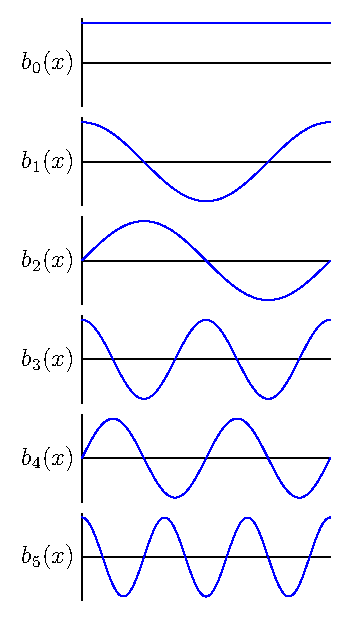
\includegraphics[width=0.9\linewidth]{fourier}\\
      \vspace*{1cm}
      \includegraphics[width=0.9\linewidth]{R3}
    \end{center}
  \end{minipage}
\end{PauseHighLight}

\end{slide}



%%%%%%%%%%%%%%%%%%%%%%% Next Slide %%%%%%%%%%%%%%%%%%%%%%%

\begin{slide}
\section{Algebraic Structure}

\begin{PauseHighLight}
  \begin{itemize}
  \item We have gone to these lengths as we want to show that many
    properties of vectors are shared by other objects (matrices,
    functions, etc.)\pause
  \item Mathematicians study \textit{algebraic structures} such as
    vector spaces, metric spaces, Hilbert spaces (infinite dimensional
    spaces with a norm and an inner product)\pause
  \item Many of the concepts (distance/metric, norms, inner products)
    will re-occur many times within the course\pause
  \end{itemize}
\end{PauseHighLight}

\end{slide}

%%%%%%%%%%%%%%%%%%%%%%% Next Slide %%%%%%%%%%%%%%%%%%%%%%%
\Outline % Operators
%%%%%%%%%%%%%%%%%%%%%%% Next Slide %%%%%%%%%%%%%%%%%%%%%%%

\begin{slide}
\section{Operators}

\begin{PauseHighLight}
  \begin{itemize}
  \item In machine learning we are interested in transforming our input
    vectors into some output predictions\pause
  \item To accomplish this we will apply some mapping or operators on
    the vector $\mathcal{T}: \mathcal{V} \rightarrow \mathcal{V}'$\pause
  \item This says that $\mathcal{T}$ maps some object
    $\bm{x}\in\mathcal{V}$ to an object $\bm{y}=\mathcal{T}[\bm{x}]$ in
    a new vector space $\mathcal{V}'$\pause
  \item This new vector space may or may not be the same as the original
    vector space\pause
  \item Our objects may be any object in a vector space such as a
    function\pause
  \end{itemize}
\end{PauseHighLight}

\end{slide}

%%%%%%%%%%%%%%%%%%%%%%% Next Slide %%%%%%%%%%%%%%%%%%%%%%%

\begin{slide}
\section{Linear Operators}

\begin{PauseHighLight}
  \begin{itemize}
  \item Operators are in general very complicated, but a particular nice set
    of operators are linear operators\pause
  \item $\mathcal{T}$ is a linear operator if
    \begin{enumerate}
    \item $\mathcal{T}[a\,\bm{x}] = a\,\mathcal{T}[\bm{x}]$
    \item $\mathcal{T}[\bm{x} + \bm{y}] = \mathcal{T}[\bm{x}] +
      \mathcal{T}[\bm{y}]$\pause
    \end{enumerate}
  \item For normal vectors the most general linear operation is
    \begin{align*}
      \mathcal{T}[\bm{x}] = \mat{M}\,\bm{x}
    \end{align*}
  where $\mat{M}$ is a matrix\pause
  \end{itemize}
\end{PauseHighLight}

\end{slide}

%%%%%%%%%%%%%%%%%%%%%%% Next Slide %%%%%%%%%%%%%%%%%%%%%%%

\begin{slide}
\section[-2]{Matrix multiplication}

\begin{PauseHighLight}
  \begin{itemize}
  \item For an $\ell \times m$ matrix $\mat{A}$ and an $m \times n$
    matrix $\mat{B}$ we can compute the ($\ell\times n$) product, $\mat{C} =
    \mat{A}\,\mat{B}$, such that
    \begin{align*}
      C_{ij} = \sum_{k=1}^m A_{ik}\,B_{kj}\pause \hspace{2cm}
      \raisebox{-1cm}{\includegraphics[width=0.3\linewidth]{matrixMult}}
    \end{align*}
  \item Treating the vector $\bm{x}$ as a $n\times1$ matrix then
    \begin{align*}
      \bm{y} = \mat{A}\, \bm{x} \quad \Rightarrow \quad y_i = \sum_{j}
      M_{ij} x_j\pause \hspace{2cm}
      \raisebox{-1cm}{\includegraphics[width=0.27\linewidth]{matrixVector}}
    \end{align*}
  \item Using the same matrix notation we can define the inner product
    as
    \begin{align*}
      \langle \bm{x}, \bm{y} \rangle = \bm{x}^\tr \bm{y} = \sum_{i=1}^n
      x_i\,y_i \pause \hspace{2cm}
      \raisebox{-1cm}{\includegraphics[width=0.25\linewidth]{dotProduct}}
    \end{align*}
  \end{itemize}
\end{PauseHighLight}

\end{slide}

%%%%%%%%%%%%%%%%%%%%%%% Next Slide %%%%%%%%%%%%%%%%%%%%%%%

\begin{slide}
\section{Kernels}

\begin{PauseHighLight}
  \begin{itemize}
  \item The equivalent of a matrix for functions (i.e. a linear
    operator) is known as a kernel $K(x,y)$
    \begin{align*}
      g(x) = \mathcal{T}[f] = \int_{y\in\mathcal{I}} K(x,y)\, f(y) \,
      \dd y\pause
    \end{align*}
  \item Our domain does not need to be one dimensional, e.g.
    \begin{align*}
      g(\bm{x}) = \mathcal{T}[f] = \int_{\bm{y}\in\mathcal{I}}
      K(\bm{x},\bm{y})\, f(\bm{y}) \, \dd \bm{y}\pause
    \end{align*}
  \item We shall soon see examples of high-dimensional kernels\pause
  \end{itemize}
\end{PauseHighLight}

\end{slide}

%%%%%%%%%%%%%%%%%%%%%%% Next Slide %%%%%%%%%%%%%%%%%%%%%%%

\begin{slide}
\section[-1]{Kernels in Machine Learning}

\begin{PauseHighLight}
  \begin{itemize}
  \item Kernels are used heavily in machine learning\pause
  \item In kernel methods such as SVM, SVR, Kernel-PCA\pause
  \item They are also used in Gaussian Processes\pause
  \item In all these cases we consider symmetric, positive
    semi-definite kernels\pause
  \item Sometimes they can be interpreted as covariance between random functions
    \begin{align*}
      K(\bm{x},\bm{y})
      = \av[f\sim\mathcal{P}]{\left(\strut f(\bm{x})-\mu(\bm{x})\right)
      \left(\strut f(\bm{y})-\mu(\bm{y})\right)}\pause
    \end{align*}
  \end{itemize}
\end{PauseHighLight}


\end{slide}

%%%%%%%%%%%%%%%%%%%%%%% Next Slide %%%%%%%%%%%%%%%%%%%%%%%

\begin{slide}
\section[-2]{General Linear Mappings}

\pb\pause\pauselevel{=1}
\begin{itemize}
\item In general a linear operator will map vectors between different
  vector spaces\pauseh
\item E.g. $\mathbb{R}^3 \rightarrow \mathbb{R}^2$\pauseh\pauselevel{=1 =2}
  \begin{center}
    \multipdf[width=0.8\linewidth]{generalMap}\pause
  \end{center}
\end{itemize}


\end{slide}

%%%%%%%%%%%%%%%%%%%%%%% Next Slide %%%%%%%%%%%%%%%%%%%%%%%

\begin{slide}
\section{Square Matrices}

\begin{PauseHighLight}
  \begin{itemize}
  \item We will spend a lot of time on operators that map from a vector
    space onto itself $\mathcal{T}: \mathcal{V}\rightarrow\mathcal{V}$\pause
  \item For vectors in $\mathbb{R}^n$ such linear operators are
    represented by square matrices\pause
  \item When there is a one-to-one mapping then we have a unique inverse\pause
  \item We will study such mappings in detail in the next lecture\pause
  \end{itemize}
\end{PauseHighLight}

\end{slide}

%%%%%%%%%%%%%%%%%%%%%%% Next Slide %%%%%%%%%%%%%%%%%%%%%%%

\begin{slide}
\section{Summary}

\begin{PauseHighLight}
  \begin{itemize}
  \item We haven't covered much machine learning as
    such\pause---sorry\pauseb
  \item But mathematics is the language of machine learning and you have
    to get used to it\pause
  \item Mathematics is like programming, if you don't understand the
    syntax and you can't write it down then its meaningless\pause
  \item We've taken a high level view of vector spaces, this will pay us
    back later as we look at kernel methods\pause
  \end{itemize}
\end{PauseHighLight}

\end{slide}


%%% Local Variables:
%%% TeX-master: "lectures"
%%% End:
